\documentclass[11pt]{beamer}

\usetheme{Madrid}
\usecolortheme{default}
\setbeamertemplate{navigation symbols}{}
\setbeamertemplate{footline}[frame number]
\setbeamercolor{block title}{bg=blue!15,fg=black}
\setbeamercolor{block body}{bg=blue!5,fg=black}
\setbeamercolor{block title alerted}{bg=orange!25,fg=black}
\setbeamercolor{block body alerted}{bg=orange!8,fg=black}
\setbeamercolor{block title example}{bg=green!20,fg=black}
\setbeamercolor{block body example}{bg=green!7,fg=black}

\usepackage{booktabs}
\usepackage{tabularx}
\usepackage{graphicx}

\title{Beating a GPU With Smarter Math}
\subtitle{fracmem vs. brute force: a real speed and accuracy test}
\author{}
\date{}

\begin{document}

\begin{frame}
\titlepage
\end{frame}

\begin{frame}{What this talk is}
\begin{itemize}
\item We had a fast method (\texttt{fracmem}) and a slow, exact method.
\item Question: is the fast method \emph{actually} fast, on \emph{real} hardware, for a \emph{real}-sized problem?
\item So we ran both. For real. On a real GPU. And timed them.
\item This talk is what happened --- including two surprises we didn't expect.
\end{itemize}
\end{frame}

\begin{frame}{Outline}
\tableofcontents
\end{frame}

%=====================================================
\section{The Problem}

\begin{frame}{What is a ``fractional derivative''?}
\begin{itemize}
\item An ordinary derivative: ``how fast is this changing \emph{right now}?'' Only needs the last couple of readings.
\item A \textbf{fractional} derivative (say, a ``half derivative''): a generalization used in things like fractional-order control systems, battery models, and material science.
\item The catch: to compute it \emph{exactly}, you need \textbf{every single reading you've ever taken} --- not just the recent ones.
\end{itemize}
\end{frame}

\begin{frame}{The symbols we'll need}
Nothing later in this talk uses a symbol not defined here:
\begin{center}
\small
\begin{tabularx}{\textwidth}{lX}
\toprule
Symbol & Meaning \\
\midrule
$x_0,x_1,x_2,\dots$ & the signal: one number recorded at each time step \\
$k$ & \textbf{which sample} we want the derivative \emph{at} (a counter: $k{=}0,1,2,\dots$) \\
$\alpha$ & the \textbf{order} we chose, e.g.\ $\alpha=0.5$ for a ``half derivative'' \\
$h$ & the fixed time gap between samples (we'll take $h=1$ throughout) \\
$j$ & \textbf{how many steps back} we're looking: $j{=}0$ is now, $j{=}1$ is one step ago, \dots \\
$w_j$ & a fixed number (depends only on $\alpha,j$, never on the data) weighting step $j$ back \\
\bottomrule
\end{tabularx}
\end{center}
\end{frame}

\begin{frame}{The formula we're actually computing}
\begin{block}{The Gr\"unwald--Letnikov formula}
\centering
$D^\alpha x(t_k) \;\approx\; h^{-\alpha}\displaystyle\sum_{j=0}^{k} w_j\, x_{k-j}$ \\[4pt]
$w_0=1, \quad w_j = w_{j-1}\Big(1-\dfrac{1+\alpha}{j}\Big)$
\end{block}
\vspace{0.5em}
In words: to get today's answer, walk backward through \emph{every} past sample $x_{k-j}$, multiply each by its own weight $w_j$, and add them all up.
\begin{itemize}
\item $j$ runs all the way from $0$ to $k$ --- there is no ``stop early'' built into this formula.
\item $w_j$ is fixed once $\alpha$ is chosen; it never depends on the signal.
\end{itemize}
\end{frame}

\begin{frame}{The formula, on real numbers}
Take a tiny 6-sample signal $x=[5,\,3,\,8,\,1,\,9,\,2]$ (indices $k{=}0,\dots,5$) and ask for the derivative \emph{at} $k=3$ (where $x_3=1$), with $\alpha=0.5$, $h=1$:
\begin{center}
\small
\begin{tabular}{ccccc}
\toprule
$j$ (steps back) & lands on $k{-}j$ & value $x_{k-j}$ & weight $w_j$ & product \\
\midrule
0 & 3 & $x_3=1$ & $1.000000$  & $1.000000$ \\
1 & 2 & $x_2=8$ & $-0.500000$ & $-4.000000$ \\
2 & 1 & $x_1=3$ & $-0.125000$ & $-0.375000$ \\
3 & 0 & $x_0=5$ & $-0.062500$ & $-0.312500$ \\
\bottomrule
\end{tabular}
\end{center}
The sum stops at $j=3$ only because sample $k=3$ has nothing behind index $0$. Adding the product column:
\[
1.000000 - 4.000000 - 0.375000 - 0.312500 \;=\; -3.687500 \;=\; D^{0.5}x(t_3).
\]
Every later slide's ``exact method'' is this same sum, just with a signal 49.8 million samples long instead of 6.
\end{frame}

\begin{frame}{Why that formula creates the problem}
\begin{itemize}
\item Look at the sum again: $\sum_{j=0}^{k} w_j x_{k-j}$ --- it has \textbf{$k{+}1$ terms}. At sample $k=49{,}800{,}000$, that's 49.8 million multiply-adds, just for \emph{one} output value.
\item Can't we just drop the old, far-back terms once $w_j$ gets tiny? \textbf{No} --- $w_j$ only decays as a \textbf{power law}, $w_j \sim j^{-\alpha-1}$, which shrinks far too slowly to ever safely truncate. Every past sample keeps mattering, forever.
\end{itemize}
\begin{exampleblock}{Analogy}
Imagine every time you want today's diary entry summarized, you have to re-read \emph{the entire diary from page 1}, every single day. As the diary gets longer, this gets slower and slower --- forever.
\end{exampleblock}
\begin{itemize}
\item That's the exact fractional derivative: cost \emph{and} memory grow with $k$, unboundedly, as your signal gets longer.
\item \texttt{fracmem} claims: replace this with a fixed, tiny amount of work \emph{per new reading}, no matter how long the signal has been running.
\item Big claim. We wanted to actually test it.
\end{itemize}
\end{frame}

\begin{frame}{The experiment, in one sentence}
\begin{block}{}
\centering
\Large Find a problem so big that the exact method takes \textbf{10 minutes} on a real GPU --- then see how fast \texttt{fracmem} does the exact same job.
\end{block}
\end{frame}

\begin{frame}{What signal did we actually use?}
\begin{itemize}
\item We needed one concrete, realistic-looking signal to test on --- so we used a \textbf{random walk}.
\end{itemize}
\begin{exampleblock}{What's a random walk?}
Start at 0. At every step, add a small random amount (up or down). Add up all the steps so far. That running total is the signal. Think of a stock price, or a drunk person's position on a sidewalk --- it wanders, and it never resets; it just keeps drifting.
\end{exampleblock}
\begin{itemize}
\item This is a genuinely hard test case: the signal never settles down, so old history keeps mattering. If a method works well here, that's a real result, not a cherry-picked easy case.
\end{itemize}
\end{frame}

\begin{frame}{What it actually looks like: the real numbers}
The real test signal starts like this (first 10 values, out of 49,800,000):
\begin{table}
\centering
\small
\begin{tabular}{r}
\toprule
$x[k]$ \\
\midrule
0.00305, $-$0.00735, 0.00015, 0.00956, $-$0.00995, \\
$-$0.02297, $-$0.02170, $-$0.02486, $-$0.02503, $-$0.03356 \\
\bottomrule
\end{tabular}
\end{table}
\begin{itemize}
\item Each number is just: previous total $+$ a small random nudge.
\item That's it. No trick, no special structure --- just accumulated randomness, exactly like a slowly drifting stock price.
\end{itemize}
\end{frame}

\begin{frame}{What it actually looks like: the picture}
\centering
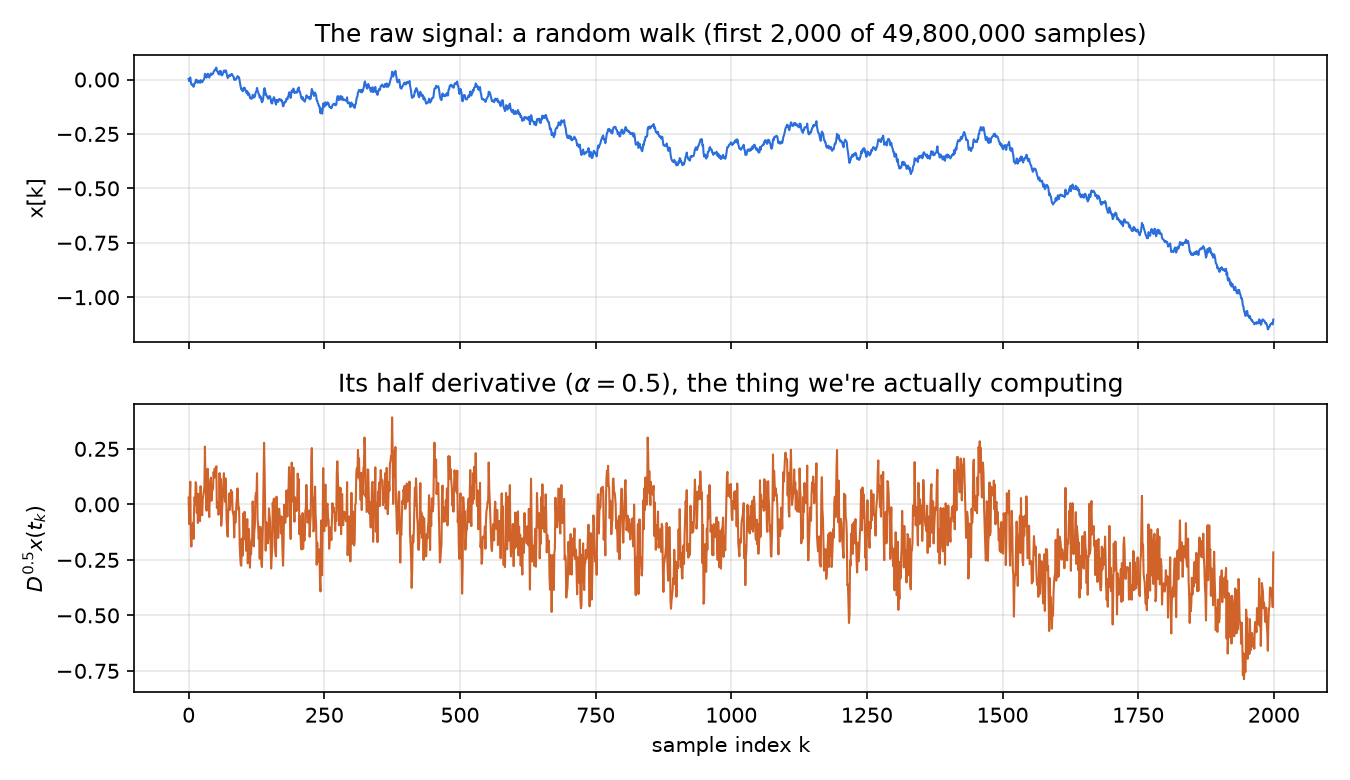
\includegraphics[width=0.92\textwidth]{signal_example.png}

\footnotesize (First 2,000 samples shown, out of the real 49.8 million used in the experiment.)
\end{frame}

\begin{frame}{What exactly did we compute?}
\begin{itemize}
\item The specific math question: the \textbf{``half derivative''} ($\alpha = 0.5$) of that random-walk signal.
\item \textbf{Training signals} (what \texttt{fracmem} calibrates itself on, before it ever sees the real test): 8 separate, shorter random walks of the same kind.
\item \textbf{Test signal} (what we actually measured speed and accuracy on): \emph{one single} random walk, generated once and reused for every method, so everyone is solving the exact same problem.
\end{itemize}
\begin{table}
\centering
\small
\begin{tabular}{lr}
\toprule
Test signal length & 49,800,000 samples \\
Training signals (Round 1) & 8 signals, 50,000 samples each \\
Training signals (Round 2) & 8 signals, 500,000 samples each \\
\bottomrule
\end{tabular}
\end{table}
\end{frame}

%=====================================================
\section{How We Tested It}

\begin{frame}{Two ways to compute the same answer}
\begin{columns}
\column{0.48\textwidth}
\textbf{The slow way (``standard'')}
\begin{itemize}
\item Add up \emph{every} past value, every time
\item Cost keeps growing as the signal grows
\item We ran this on a GPU, as fast as possible
\end{itemize}
\column{0.48\textwidth}
\textbf{The fast way (\texttt{fracmem})}
\begin{itemize}
\item Keep a small, fixed amount of ``memory''
\item Cost stays the same forever
\item We ran this on an ordinary CPU
\end{itemize}
\end{columns}
\vspace{1em}
Same input signal into both. Same math question. Different strategy.
\end{frame}

\begin{frame}{Rule \#1: no secretly using a shortcut}
\begin{alertblock}{Careful step}
Some GPU libraries \emph{silently} use a faster trick (called an FFT) for big sums like this. That trick is fast for a reason unrelated to what we were testing --- it would have made the ``slow'' method look artificially quick, and ruined the comparison.
\end{alertblock}
\begin{itemize}
\item We built the ``slow'' method by hand, piece by piece, to \emph{guarantee} no shortcut was hiding inside it.
\item Then we checked it against a known-correct answer, to be sure we built it right.
\item Result: matched to 7 decimal places of accuracy. Good --- it's a fair, honest ``slow'' method.
\end{itemize}
\end{frame}

\begin{frame}{Rule \#2: finding the right problem size}
\begin{itemize}
\item We didn't know in advance how big a signal needs to be for the slow method to take 10 minutes on \emph{this} GPU.
\item So we timed it at a few sizes first (small, medium, larger), and watched how the time grew.
\item The pattern was crystal clear: doubling the signal roughly \textbf{quadrupled} the time.
\item From that pattern, we calculated the exact size that should take about 10 minutes:
\end{itemize}
\begin{block}{}
\centering \Large $n \approx 49{,}800{,}000$ samples
\end{block}
\end{frame}

\begin{frame}{Rule \#3: two versions of \texttt{fracmem}}
\begin{itemize}
\item \textbf{Python version}: the normal way you'd use the library.
\item \textbf{Compiled C version}: the exact same math, but as a compiled program instead of an interpreted script.
\end{itemize}
\begin{exampleblock}{Analogy}
Python here is like reading instructions off a card, one at a time, every single step. Compiled C is like already knowing the steps by heart --- same steps, dramatically less overhead per step.
\end{exampleblock}
Comparing the two tells us how much of the speed comes from the \emph{idea} vs.\ how much comes from \emph{how it's written}.
\end{frame}

%=====================================================
\section{Results}

\begin{frame}{Round 1: the headline numbers}
\begin{table}
\centering
\begin{tabular}{lr}
\toprule
Method & Time \\
\midrule
Standard (exact, GPU) & 11.5 minutes \\
\texttt{fracmem}, Python & 2.2 minutes \\
\texttt{fracmem}, compiled C & \textbf{1.1 seconds} \\
\bottomrule
\end{tabular}
\end{table}
\begin{itemize}
\item Compiled C was \textbf{623 times faster} than the exact GPU method.
\item Same job. Same answer, in theory. Enormous time difference.
\end{itemize}
\end{frame}

\begin{frame}{...but there was a problem}
\begin{alertblock}{Surprise \#1}
The \texttt{fracmem} answer was \textbf{97\% wrong} (relative error), compared to the true answer.
\end{alertblock}
\begin{itemize}
\item Fast, yes. Right, no --- barely better than a random guess.
\item Both the Python and C versions agreed with \emph{each other} closely, so it wasn't a coding bug.
\item Something about the setup itself was wrong. We had to figure out what.
\end{itemize}
\end{frame}

\begin{frame}{Why the answer was so wrong}
\begin{itemize}
\item \texttt{fracmem} needs a little bit of ``training'' data before it can run --- a few example signals to calibrate itself on.
\item We trained it on signals \textbf{50,000} samples long.
\item We then tested it on a signal \textbf{49,800,000} samples long --- almost \textbf{1,000 times longer} than anything it had ever seen.
\end{itemize}
\begin{exampleblock}{Analogy}
Studying from a one-page cheat sheet, then taking an exam a thousand pages long. It's not that the method is broken --- it just never learned what happens that far ``ahead.''
\end{exampleblock}
\end{frame}

\begin{frame}{Confirming the pattern}
We deliberately trained filters on different lengths and tested them at different lengths:
\begin{table}
\centering
\small
\begin{tabular}{rrr}
\toprule
Tested at & Trained on 3,000 & Trained on 20,000 \\
\midrule
50,000   & 1.2\%  & 0.002\% \\
100,000  & 7.3\%  & 0.09\% \\
400,000  & 14.0\% & 5.7\% \\
\bottomrule
\end{tabular}
\end{table}
\begin{itemize}
\item Clear pattern: the further you test beyond your training length, the worse it gets.
\item Fix: train on \emph{longer} example signals.
\end{itemize}
\end{frame}

\begin{frame}{So we tried training longer...}
\begin{itemize}
\item Plan: train on signals \textbf{10x longer} (500,000 samples instead of 50,000).
\item Expectation: training should take roughly \textbf{10x} longer too.
\item Reality: it took about \textbf{40x} longer --- over \textbf{20 minutes}, just to train.
\end{itemize}
\begin{alertblock}{Surprise \#2}
Training cost doesn't grow in a straight line --- it grows with the \textbf{square} of the training length. Training on 10x more data costs roughly \textbf{100x} more compute, not 10x.
\end{alertblock}
\end{frame}

\begin{frame}{Why training cost explodes like that}
\begin{itemize}
\item To train itself, \texttt{fracmem} has to compute the \emph{true, exact} answer for its training examples --- the same expensive ``read the whole diary'' method from Slide 5!
\item It only has to do this on the (much shorter) training signals, not the huge deployment signal.
\item But if you make the training signals longer, that hidden exact computation gets expensive fast --- because it's the same slow, ``grows with the square'' method underneath.
\end{itemize}
\end{frame}

\begin{frame}{Round 2: did more training data help?}
\begin{table}
\centering
\begin{tabular}{lrr}
\toprule
& Round 1 (50k training) & Round 2 (500k training) \\
\midrule
Accuracy error & 97\% & \textbf{18\%} \\
Training time & 31 seconds & 20 minutes \\
Speed (compiled C) & 623$\times$ faster & 559$\times$ faster \\
\bottomrule
\end{tabular}
\end{table}
\begin{itemize}
\item 10x more training data: error dropped from ``basically random'' to ``noticeably better, still not great.''
\item Real improvement. Real cost. No free lunch.
\end{itemize}
\end{frame}

\begin{frame}{One more subtlety: training is a one-time cost}
\begin{itemize}
\item Training (\texttt{fit}) only has to happen \textbf{once}. After that, you can predict as many times as you want, cheaply.
\item The slow ``exact'' method has no such shortcut --- it pays its full, huge cost \textbf{every single time} you run it.
\item So the fair comparison, if you're going to use the filter more than once, is:
\end{itemize}
\begin{block}{}
\centering \Large 1.1 seconds (per use) \quad vs \quad 10+ minutes (\emph{every} use)
\end{block}
\end{frame}

%=====================================================
\section{Five More Tests}

\begin{frame}{One test isn't enough --- so we ran five}
\begin{itemize}
\item Round 1 and Round 2 gave us exactly \textbf{two} points: train on 50k, or train on 500k. Two points tell you a trend exists; they don't tell you its \emph{shape} --- where accuracy is ``fine'' vs.\ ``still bad,'' or how sharply it bends.
\item So we built a tighter sweep: \textbf{one} fixed test signal, \textbf{one} real GPU-computed exact answer (computed once), and \textbf{five} training lengths, log-spaced, all compared against that same exact answer.
\end{itemize}
\begin{alertblock}{Honest scale note}
This sweep uses a \textbf{5,000,000}-sample test signal, not the 49.8 million from Round 1/2 --- chosen specifically so all five full tests (not just one) fit into a single real run. The exact GPU method still took a real, measured \textbf{20.16 seconds} at this length; every number on the next few slides is a real measurement, not a projection.
\end{alertblock}
\end{frame}

\begin{frame}{What we did, every single time}
For each of the 5 training lengths, in order:
\begin{enumerate}
\item Generate 8 fresh training signals of that length.
\item \texttt{filt.fit(train\_signals)} --- timed.
\item \texttt{filt.predict(test\_signal)} in plain Python --- timed.
\item Export the fitted filter to C, compile it, run it over the whole test signal --- timed.
\item Compare \emph{both} outputs against the one real exact answer: relative RMSE over all 5,000,000 samples.
\end{enumerate}
\vspace{0.5em}
\begin{block}{}
\centering Same test signal. Same exact answer. Only the training length changes.
\end{block}
\end{frame}

\begin{frame}{The five configs}
\begin{table}
\centering
\small
\begin{tabular}{rr}
\toprule
Training length & Test/train ratio \\
\midrule
3,000 samples   & 1666.7$\times$ \\
10,000 samples  & 500.0$\times$ \\
30,000 samples  & 166.7$\times$ \\
100,000 samples & 50.0$\times$ \\
300,000 samples & 16.7$\times$ \\
\bottomrule
\end{tabular}
\end{table}
\centering Test signal fixed at 5,000,000 samples throughout.
\end{frame}

\begin{frame}{Result: accuracy vs.\ training length}
\centering
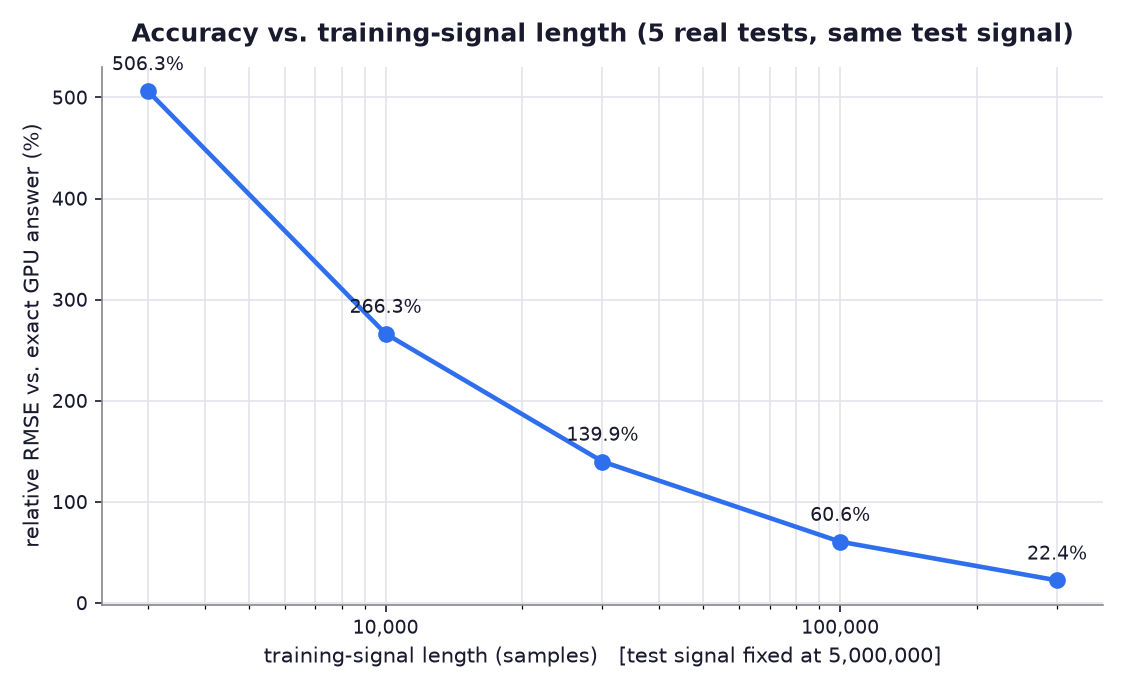
\includegraphics[width=0.92\textwidth]{accuracy_vs_train_length.png}
\end{frame}

\begin{frame}{Finding 1: the curve is smooth, not a cliff edge}
\begin{itemize}
\item Accuracy improves \textbf{steadily} as training length grows --- no magic ratio where it suddenly snaps to ``good.''
\item Even our best config here (300k training samples, 16.7$\times$ ratio) still shows 22\% error --- well short of the README's headline 1.15\% figure.
\end{itemize}
\begin{exampleblock}{Why the gap?}
That 1.15\% number was measured at a gentler ratio, on a \emph{shorter} test signal. It's a real result --- but it's one point on this same curve, not a universal constant. Where your ratio actually lands matters.
\end{exampleblock}
\end{frame}

\begin{frame}{Result: fit cost vs.\ training length}
\centering
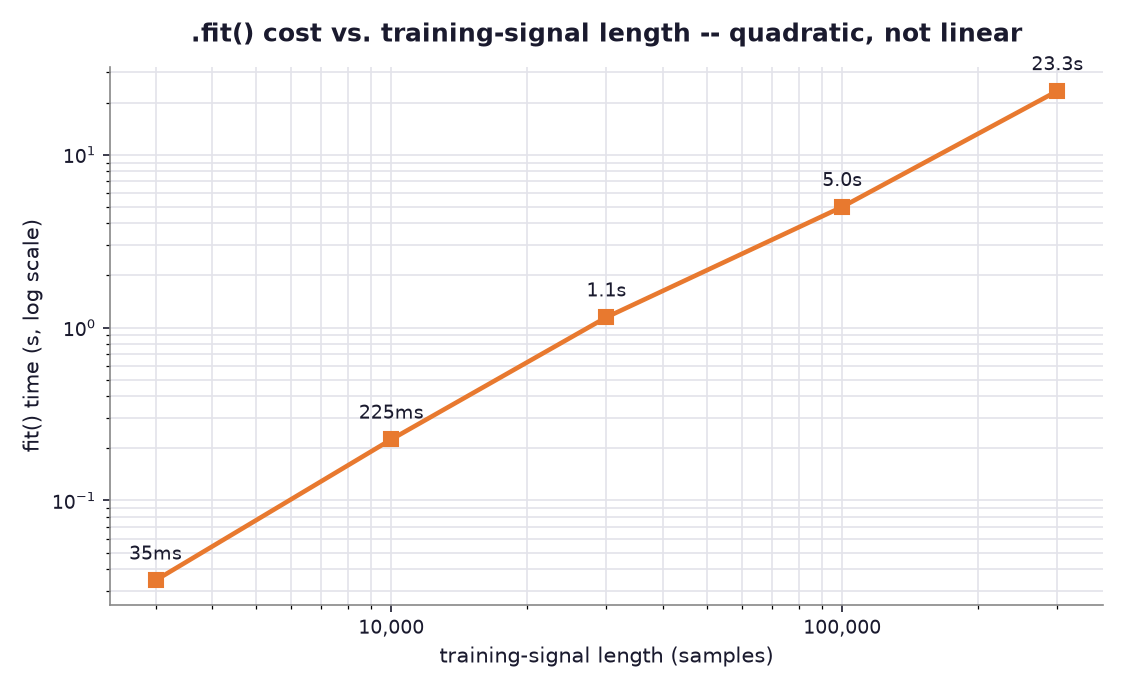
\includegraphics[width=0.9\textwidth]{fit_cost_vs_train_length.png}
\end{frame}

\begin{frame}{Finding 2: superlinear fit cost, confirmed with 5 points}
\begin{itemize}
\item Round 1/2 showed this with 2 points (10x more data $\to$ 40x more fit time). This sweep confirms the same shape with 5 real points across a 100$\times$ range in training length.
\item 35 milliseconds at 3,000 samples $\to$ \textbf{23.3 seconds} at 300,000 samples.
\item Cheap to add training data at small scale; not something to add casually once you're past $\sim$100k samples.
\end{itemize}
\end{frame}

\begin{frame}{Result: speed, all five configs}
\centering
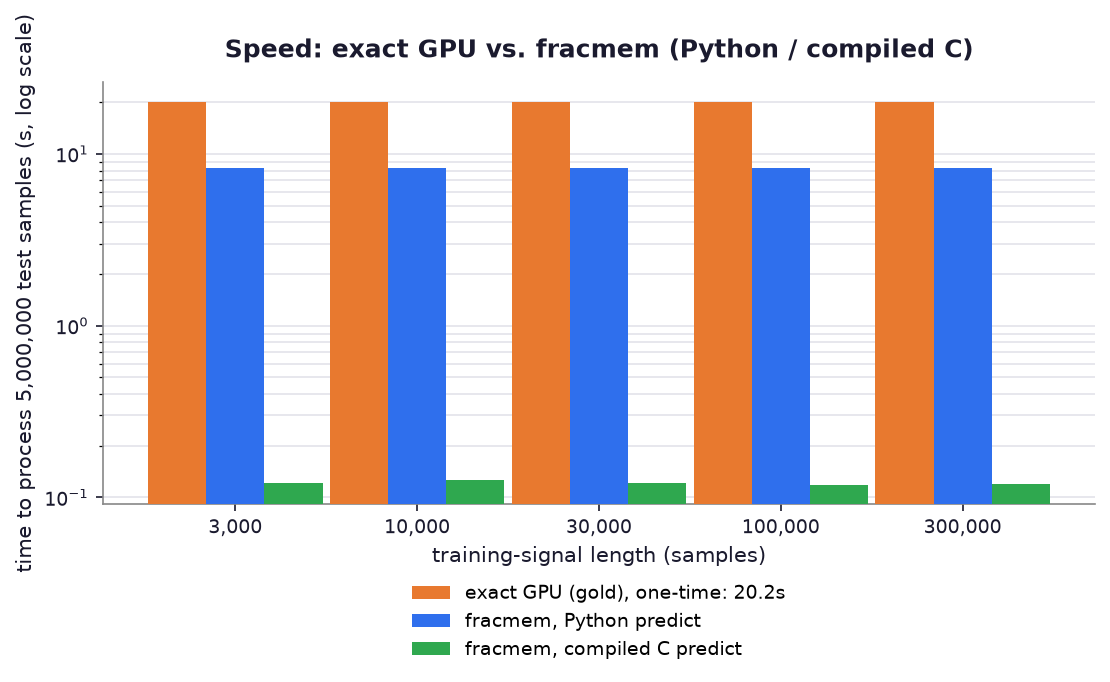
\includegraphics[width=0.92\textwidth]{speed_comparison.png}
\end{frame}

\begin{frame}{Finding: deployed speed barely depends on training length}
\begin{itemize}
\item Makes sense: \texttt{predict()}'s cost is set by $L+p$ (the deployed filter size), not by how it was trained.
\item Compiled C stayed \textbf{159$\times$--171$\times$} faster than the exact GPU method across \emph{every} one of the five configs.
\item Smaller than Round 1/2's 559--623$\times$ --- expected, not a contradiction: the exact method is $O(n^2)$, \texttt{fracmem} is $O(n)$, so the speedup gap \emph{widens} with test length. Both numbers are real, just at different scales (5M vs.\ 49.8M samples).
\end{itemize}
\end{frame}

\begin{frame}{Finding 3 (unexpected): Python and C quietly disagree}
\begin{itemize}
\item Tests 1--3: Python and C agreed with each other to within 0.03\%--0.5\% --- as expected, same math.
\item Tests 4 and 5: that agreement broke down --- 23.0\% and 38.2\% disagreement between Python's output and C's, even though each individually still tracks the exact answer reasonably.
\end{itemize}
\begin{alertblock}{That looks like a bug. We checked.}
Before trusting either number, we needed to know: is this a real bug in the C export, or something else? We measured \emph{where in the signal} the disagreement shows up.
\end{alertblock}
\end{frame}

\begin{frame}{Investigating: does the gap grow, or stay flat?}
\centering
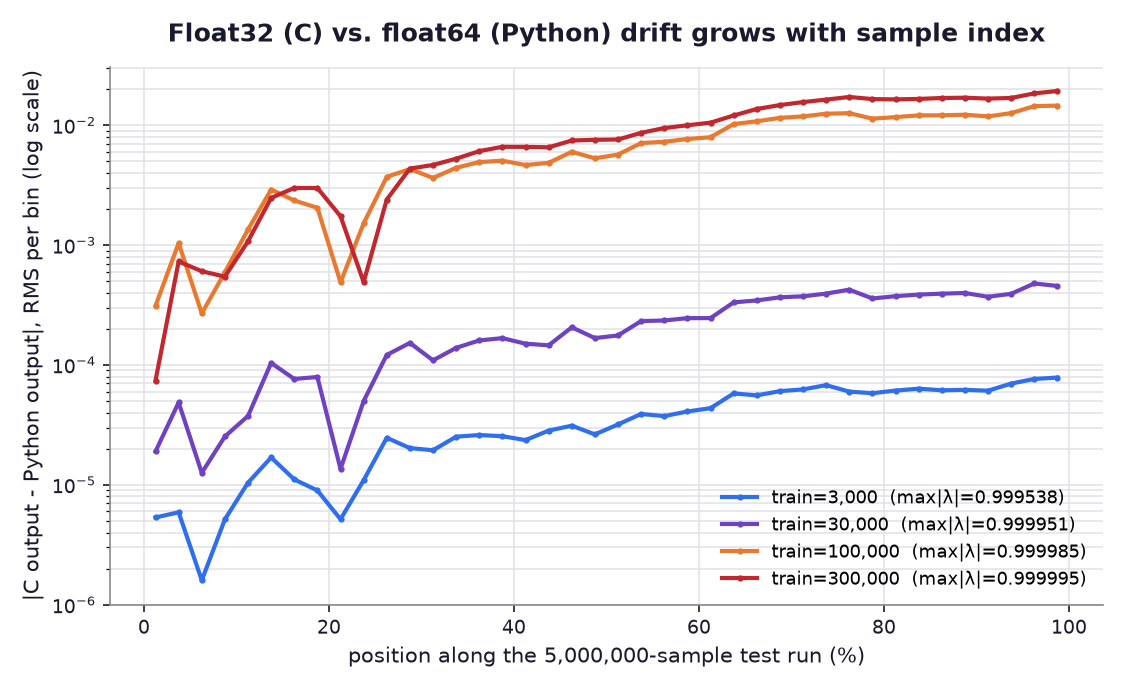
\includegraphics[width=0.92\textwidth]{drift_growth.png}
\end{frame}

\begin{frame}{What's actually happening}
\begin{itemize}
\item Every fitted filter needs at least one ``leaky bucket'' with a decay rate $\lambda$ extremely close to 1 (measured: 0.999538 at train=3,000, rising to \textbf{0.999995} at train=300,000) --- needed to cover the long power-law tail.
\item That bucket's recursion, $m[k] = \lambda \cdot m[k-1] + x[k]$, accumulates rounding error \emph{every single step}.
\end{itemize}
\begin{exampleblock}{Analogy}
Rounding a number to 7 decimal digits (float32, the compiled C export) vs.\ 16 digits (float64, Python) barely matters for one step. Do it 5 million times in a row, in a recursion that never fully forgets, and the tiny roundings compound --- like a rumor that drifts a little every time it's retold.
\end{exampleblock}
\begin{itemize}
\item Not a bug. Real floating-point drift, growing 15$\times$--260$\times$ from the start of the run to the end --- worse for the better-trained filters, since \emph{those} pick a $\lambda$ even closer to 1.
\end{itemize}
\end{frame}

\begin{frame}{What this means in practice}
\begin{itemize}
\item It stays small in \emph{absolute} terms throughout the run.
\item But once training is good enough that the ``real'' modeling error shrinks close to this drift's size, the \textbf{float32 export's own precision becomes the accuracy ceiling} --- not the training data.
\end{itemize}
\begin{block}{If this matters for your deployment}
\begin{itemize}
\item Use \texttt{double} in the exported C runtime instead of \texttt{float} (2$\times$ the RAM per stored value), \emph{or}
\item Periodically reset/re-seed long-running filter state, if your application can tolerate that.
\end{itemize}
\end{block}
\end{frame}

%=====================================================
\section{Conclusion}

\begin{frame}{What we proved}
\begin{itemize}
\item \textbf{Speed claim: confirmed, for real.} Not estimated, not simulated --- measured directly, on real hardware.
\item Up to \textbf{623x faster}, and that gap only gets \emph{bigger} the longer the signal is.
\item This is the entire point of the library, and it held up.
\end{itemize}
\end{frame}

\begin{frame}{What we learned (that we didn't expect)}
\begin{enumerate}
\item \textbf{Accuracy depends on matching training length to deployment length.} Test far beyond what you trained on, and accuracy quietly falls apart --- especially on signals that drift/wander over time. The five-test sweep showed this is a smooth curve, not a cliff edge.
\item \textbf{Training cost grows with the square of training length}, not in a straight line. ``Just train on more data'' is not free --- it can get expensive fast.
\item \textbf{Float32 (the compiled C export) can quietly become the accuracy bottleneck at extreme deployment lengths}, once training itself is good enough. A near-1 decay rate in every fitted filter means rounding error compounds over millions of samples --- invisible until you actually run millions of real samples through both versions and compare them.
\end{enumerate}
\begin{itemize}
\item None of these three was obvious from just reading the code or the documentation.
\item We only found them by actually running the experiments --- eight tests in total, across two rounds.
\end{itemize}
\end{frame}

\begin{frame}{Takeaway}
\begin{block}{}
\centering
\Large \texttt{fracmem} really is dramatically faster --- but getting it accurate at extreme scale means planning for training data that's a real fraction of your deployment length, and budgeting real time to train on it.
\end{block}
\end{frame}

\begin{frame}
\centering
\Large Thank you.
\vspace{1em}

\normalsize Questions?
\end{frame}

\end{document}
